\documentclass[12pt]{article}
\usepackage{epsfig}
\usepackage{natbib}
\usepackage{amssymb,amsmath}
\usepackage{titletoc}
\usepackage{color}
\usepackage{graphicx}
\usepackage[toc,page]{appendix}

% HOW TO SET UP AN 8.5 x 11:
% http://www.pages.drexel.edu/~pyo22/students/latexRelated/latexTutorial.html
\topmargin -1.5cm        % read Lamport p.163
\oddsidemargin -0.04cm   % read Lamport p.163
\evensidemargin -0.04cm  % same as oddsidemargin but for left-hand pages
\textwidth 16.59cm
\textheight 21.94cm 
\parskip 7.2pt           % sets spacing between paragraphs
\parindent 0pt		     % sets leading space for paragraphs

%%%%%%%%%%%%%%%%%%%%%%%%%%%%%%%%%%%%%%%%%%%%%%%%%%%%%%%%%%%%%%%%%%%%%%
% set up formatting of python code
%
% to use insert python code, you can use
% \begin{python}
% ...
% \end{python}
\usepackage{listings}
\usepackage{color} % Used for syntax highlighting.
\usepackage{textcomp} % Used for syntax highlighting.

\renewcommand{\lstlistlistingname}{Code Listings}
\renewcommand{\lstlistingname}{Code Listing}
\definecolor{gray}{gray}{0.5}
\definecolor{key}{rgb}{0,0.5,0}
\lstnewenvironment{python}[1][]{
\lstset{
language=python,
basicstyle=\ttfamily\small,
otherkeywords={1, 2, 3, 4, 5, 6, 7, 8 ,9 , 0, -, =, +, [, ], (, ), \{, \}, :, *, !},
keywordstyle=\color{blue},
stringstyle=\color{red},
showstringspaces=false,
emph={class, pass, in, for, while, if, is, elif, else, not, and, or,
def, print, exec, break, continue, return},
emphstyle=\color{black}\bfseries,
emph={[2]True, False, None, self},
emphstyle=[2]\color{key},
emph={[3]from, import, as},
emphstyle=[3]\color{blue},
upquote=true,
morecomment=[s]{"""}{"""},
commentstyle=\color{gray}\slshape,
framexleftmargin=1mm, framextopmargin=1mm, frame=shadowbox,
rulesepcolor=\color{gray},#1
}}{}
%%%%%%%%%%%%%%%%%%%%%%%%%%%%%%%%%%%%%%%%%%%%%%%%%%%%%%%%%%%%%%%%%%%%%%

\definecolor{orange}{rgb}{1.00,0.65,0.00}
\def\arcsec{^{\prime\prime}}

\newcommand{\becker} { \textcolor{orange} {
\ensuremath{\blacksquare} {\bf AndyB:}  
\ensuremath{\blacksquare} } }

\newcommand{\simon} { \textcolor{red} {
\ensuremath{\bigstar} {\bf Simon:}  
\ensuremath{\bigstar} } }

\newcommand{\ajc} { \textcolor{blue} {
\ensuremath{\clubsuit} {\bf AndyC:}  
\ensuremath{\clubsuit} } }

\newcommand{\yusra} { \textcolor{cyan} {
\ensuremath{\diamondsuit} {\bf Yusra:}  
\ensuremath{\diamondsuit} } }

\newcommand{\russ} { \textcolor{green} {
\ensuremath{\natural} {\bf Russ:}  
\ensuremath{\natural} } }

%\titlecontents{subsection}[4.8em]{}{\contentslabel{2.4em}}{\hspace*{-2.8m}}{...}
%\titlecontents{subsubsection}[6.0em]{}{\contentslabel{2.4em}}{\hspace*{-2.8m}}{}

\author{Andrew Becker, Simon Krughoff, Andrew Connolly, Yusra AlSayyad, Russ Owen}
\title{Roadmap for Winter2013 Production}
\date{\today}

\begin{document}

\maketitle

The goal of late Winter2013 production is the testing of image
subtraction algorithms and the exercise of the {\tt ip\_diffim}
package.  The package may be utilized at 3 distinct portions of the
production pipeline: in the subtraction of Snaps for the rejection of
cosmic rays; in the matching of input images for a Psf--matched
template; and in the subtraction of this template from individual
science Exposures.

The input data will be simulated LSST images (ImSim); stretch goals
include application of the algorithms to SDSS Stripe82 data (S82).
The processing steps for the ImSim data include: application of the
Isr pipeline; combining the two Snaps in a Visit into a single
Exposure; calibration, detection, and measurement on the Exposure;
stacking of multiple Exposures into a Psf--matched template image;
subtraction of this template from single--epoch Exposures; detection,
measurement, and characterization of DiaSources that remain in the
difference image; and ingestion of these DiaSources into a MySQL
database.  The natural QA hooks are in the assessment of the
Psf--matched template, and in the purity of the DiaSource sample.  We
will focus on the following metrics to assess the production:
\begin{itemize}
\item rate of false positives
\item rate of missed detections
\item performance (computational and I/O)
\end{itemize}
This document outlines the details of each stage of production,
including estimates of compute time, and addresses the anticipated
Configs for each Task.

\clearpage
\tableofcontents
\clearpage

%%%%%%%

\clearpage 
\section{ImSim Input Data} \ajc

The sets of simulated images produced for Summer 2012 (which will be
the inputs for Winter 2013 late production) are described at \\{\tt
  http://dev.lsstcorp.org/trac/wiki/ImSim/Summer2012Plan}.  Processing
of SDSS Stripe82 data is a stretch goal for Winter 2013 production.

We wish to explore the capabilities of the image subtraction software
across the focal plane, and as a function of wavelength (both of the
sources and of the effective filter).  The former argues for
operations on (at a minimum) full quadrants of the focal plane, as
vignetting is known to attenuate the signal in the outer rafts.  The
latter argues for the analysis of observations in multiple passbands:
one band where chromatic effects are expected to be negligible
($i$--band) and one where the chromatic effects are expected to be
substantial ($g$--band).

The ImSim {\tt 5yr Run} simulated 2500 visits (full focal plane) of 5
adjacent fields over a 5-year period in the full suite of filters.
The simulations include both rotational and pointing dithering, and
the atmosphere includes no clouds or aerosols.  We will extract all of
the $i$--band data of the central field for a baseline study of the
image subtraction algorithms.  The $i$--band data will serve as a
reference set that maps out the underlying performance of the
algorithms in a regime where differential chromatic refraction (DCR)
within the bandpass is expected to be negligible.  The baseline spec
will be to generate a template image from the coaddition of the first
half of these data, with the appropriate cuts on conditions and
quality.  The second half of these data will be differenced with this
template, and the quality of the subtractions analyzed based on the
metrics above.  There are {\bf XX} $i$--band images of the central
field.

We will step through several sub--production runs to assess the
quality of the processing.  This includes sub--productions runs in the
following configurations:
\begin{itemize}
\item Images in $i$-band at low airmass to avoid the effects of DCR
\item Images in $i$-band over a short timescale to avoid proper motion effects
\end{itemize}

The second portion of production will move to the analysis of data in
the $g$--band, where DCR within the passband is expected at the scale
of the Psf.  This will inform future specifications for
color--dependent Psf--modeling and Psf--matching kernels.  There are
{\bf XX} $g$--band images of the central field.

Data will be prepared at various locations and stored at JHU with
images brought over as needed.  We can use standard grid copy tools
(gridftp, bbcp).  Before large runs start, the data will need to
staged at the compute center.  The estimated time of transfer is
(We'll need to benchmark this) demonstrated rate of {\bf XXX b/s} and
ImSim data volume of {\bf XXX GB} results in transfer time of {\bf
  XXX} days.  The registry generation time is ~10min per visit.  We
will need to solve the problem of how to point to the correct flat in
the registry given a rotator angle for the science image.  This has
not been done before.

We will be applying overscan correction, bias correction and flat
fielding to the ImSim data.  The dark current in the models is below
the level we need to worry about.  The flats will be normalized to a
global value.  The zeropoints should be consistent from chip to chip.
We {\it will} need rotation dependent flats due to vignetting.
Informed by John P. we should have flats in increments of 5 deg from 0
to 90.  Amps will be assembled in readout order such that the serial
transfer direction is along the x-axis of the image.

Master flats, darks, and biases will be produced by coadding 10
examples (each including 2 snaps).  We will not be simulating any time
dependent effects in the calibration products.

The spider introduces asymmetric vignetting.  This should be taken out
using flat fields produced with a variety of rotator angles.  Where
the effect is strongest, the angular dependence introduces scatter of
$\sim~5$\%.  Using flats generated at increments of 5 deg from 0 - 90
deg (18 master flats) should bring this below the nominal 1\% error
(although any remaining error will be systematic).

John will change the simulator to produce the chips in readout order
instead of camera coordinates so that the orientation of the eimage is
synchronized with the assembled calexps.

\subsection{Issues}

The calibration production will be non-trivial.  We'll need to make
registries for $\sim~200$ visits and process them at $\sim~$minutes
per chip.  The new calibration product tasks will make this much
easier.  Simon is working on said tasks.  As of Dec 11, 2 days worth
of work before it can be submitted for review.

%%%%%%%

\clearpage 
\section{CreateCalibrationProductsTask} \simon
This work has not yet been completed.  This section is to outline the processing and needed work.  
The purpose of this task is to take individual calibration frames and combine them into
high signal to noise master frames.  Examples will be: masterbias, masterdark, masterflat, etc.  
This task will not be camera specific and will be overridden by camera specific configs (and potentially
retargetted subtasks) in the camera obs package.  The general flow of data will be to process the individual frames
with the appropriate instrument signature removal (ISR) steps for the product and camera.  Next a scale is computed for each of the input
frames.  Finally the frames are combined into the master frame.

\subsection{Input/Outputs}
Inputs are:
\begin{itemize}
\item A set of raw calibration frames.
\end{itemize}
Outputs are:
\begin{itemize}
\item A set of master calibration frames.
\end{itemize}

\subsection{CalibrationProcessTask subTask}
This is an ISR-like task that corrects the frames for the appropriate instrumental effects for that calibration
product.
\subsection{CalibrationScaleTask}
This task determines the scaling for a particular single epoch.  This task is responsible for
scaling all flats in a focal plane so that there is a single normalization for the full focalplane.
\subsection{CalibrationCombineTask}
The individual calibration frames are combined into a single high signal to noise master frame.

\subsection{Issues}
This task is relatively straight forward for the calibration products we are currently handling.  I design review will be scheduled
to address any implementation issues.


\subsection{CalibProcessTask}

%%%%%%%

\clearpage 
\section{ProcessImageTask} 
The ProcessCcdTask is does the work required to take input data from raw form all the way to a calibrated and
photometered science image.  This task is subclassed with camera specific configs and processing, but the overall 
work flow is first to do the instrument signature removal step which is handled by the camera specific subclass.  For imSim
data, there is an additional step of combining the individual snap images before the rest of processing happens. Next calibration
is run.  This measures the PSF and aperuture correction, and also does the photometric and astrometric calibration.  
Detection comes next.  After detection footprints are deblended.
Finally measurement is run on the deblended footprints.  Most of the above steps are optional, but care should be taken
when turning any one off that it does not affect down stream processing.

\subsection{Input/Outputs}
Inputs are:
\begin{itemize}
\item Raw science frame
\item Astrometry.net index files for photometric and astrometric calibration
\item Master calibration frames
\end{itemize}

Outputs are:
\begin{itemize}
\item Metadata for ingest
\item Src for ingest
\item Calexp for input to {\tt ip\_diffim}
\item Background to add to Calexp for {\tt ip\_diffim}
\item Psf for Psf matching
\end{itemize}

\subsection{IsrTask subTask}
It was decided that the instrument signature removal was so dependent on the specific instrument setup that a generalized
ISR task was not generally useful.  The ISR is expected to be handled by a camera specific task in the camera obs package.  
For imSim the process is overscan subtraction, bias correction, flat correction, assembly of amps into a ship size image, 
and interpolation of saturated and bad pixels.

\subsection{SnapCombineTask subTask} \becker

The baseline LSST observing plans defines a field ``visit'' as the
acquisition of two back--to--back images (called Snaps) and their
combination into a single visit Exposure.  The motivation for this is
to reject cosmic rays that fall outside the detection thresholds of
single--image CR rejection routines.  By subtracting the two snaps
(snap2 - snap1), CRs may be detected in the difference as objects with
either positive or negative polarity, indicating a CR in the second or
first snap, respectively.  These pixels will be masked and
interpolated, and the two snaps coadded into the final visit Exposure.

There are two options to creating the image difference on which CRs
will be detected.  The first is to take a straight difference of the
two images.  This should suffice under the assumption of a fully
realized Psf and stable atmosphere, and of sufficient precision in the
telescope tracking over the 32 second visit window.  The second option
is to use a Psf--matching kernel to register both the shapes and/or
positions of the stars if any of the assumptions above fail.  A
disadvantage of this method is that, due to the convolution inherent
in Psf--matching, the shapes of the CRs will be distorted, potentially
making them more difficult to detect.

The outstanding issue driving the decision to use Psf--matching or not
is the amount of image motion between Snaps in the W13 ImSim data.
The amplitude of these shifts in the Winter2013 test data, determined
through manual source detection and matching, is up to 0.12$\arcsec$
(0.6 pixels).  This amplitude of shift requires that image
registration techniques will be necessary for Winter2013 processing.

The Task that executes this, SnapCombine's SnapPsfMatchTask, is
configured differently than ImagePsfMatchTask, described in detail in
Section~\ref{sec-imagedifftask}, in three major ways to reflect the
prior expectation that the quality of the images is not significantly
different:

-- First the spatial order of the matching kernel is set to 0,
indicating a constant matching kernel across the image.  {\it For this
  reason we will be testing the delta--function kernel basis set in
  this environment}.  The delta--function kernel set is more sensitive
to noise than sum--of--Gaussian basis sets, but better able to model
fractional pixel shifts without significant shape distortions.  The
zero--order spatial model will help to regularize the overfitting
problem.

-- Second the size of the matching kernel is approximately half the
size of the ImagePsfMatchTask matching kernel, as the kernel power is
expected to look like an (offset) delta function.

-- Finally, we {\it will} be comparing the delta--function basis
results with a sum--of--Gaussian basis set.  However, this basis set
will be smaller than the default ImagePsfMatchTask set (31 terms).
The size of this basis set is a tuning parameter for the production
run.

After the snap difference Exposure is created, detection is run with
thresholdPolarity set to ``both''.  Measurement is then executed on
these detections.  Because these measurements will be used to mask and
interpolate pixels, it is essential that we are able to distinguish
the signal (cosmic rays) from the noise (the most significant
contaminant are the cores of bright stars).  We currently do {\it not}
have tools to reliably distinguish true cosmic rays from the cores of
bright stars in these snap differences; thus this is a core
development task for W13 processing.  We will compare the Snap
DiaSource lists to the known cosmic ray list, and to the known star
list, to establish the measurements that best separate the cosmics
from stellar cores.  Development of these query tools, and assessment
of the important distinguishing features, is an outstanding
development task.

After masking and coaddition, the visit Exposure is created.  The
combined Exposure will have an exposure time equivalent to the sum of
the two input Snaps (i.e. this will {\it not} be an average image).
The FITS keywords that need to be modified in this process include:
{\bf XXX}.  The FITS keywords that will {\it not} be modified in this
process, but that do reflect metadata that are different between the
two Snaps, include : {\bf WCS}.  These features will be copied from
the first snap of the visit pair.  The FITS keywords that will {\it
  not} be modified in this process, and that are common between the
two Snaps, include: {\bf Filter}.

\subsection{CalibrateTask subTasks} 
First off the calibration repairs any cosmic rays it finds.
The calibrate task does an initial optional background subtraction and detection phase (which also does a background background subtraction).  The detected sources are used to calculate
the PSF, the aperture correction, the photometric zeropoint, and are fed to the astrometry.net framework for astrometric
calibration.

\subsection{DetectTask subTask}
The detect task does an optional second background estimation taking into account the original detection mask set by the calibrate task.
It then runs final detection.

\subsection{DeblendTask subTask}
The deblend task searches for peaks within the footprints returned by the detect task and splits the children out into deblended sources.

\subsection{MeasureTask subTask}
The measure task makes the statistical measurements on each footprint (or peak if deblended).

\subsection{Issues}
-- A primary issue is which steps in processCcd can be turned off.  In our experience with Stripe82, we found that the products produced by
essentially all steps were necessary in later processes.  The one possible exception was the deblendTask.  Aperture corrections (CalibrateTask) 
are needed by forced photometry, zeropoints (CalibrateTask)
are needed by pipeQA and makeCoaddTask, and detection planes (DetectTask) are needed by the background matching tasks.

{\bf imSim IsrTask}
-- Saturation detection is done before bad pixel masking because we have the pixel masks in CCD coordinates.
This meant that some bad pixels were also marked as SAT.  We fix this by changing all SAT+BAD pixels back to just BAD.

-- The flats had per chip normalizations meaning that the zeropoint was not fixed for the focalplane.  This should be
fixed by the new calibration products task

{\bf SnapCombineTask}
-- The cores of bright (but not saturated) stars show up as residuals
in the Snap image difference.

-- We do not currently have tools to access the list of cosmic rays
that were input to an image (locations, shapes and amplitudes).

\subsection{New Development Tasks}

{\bf SnapCombineTask}
-- Develop tools to compare Snap DiaSources with the known cosmic ray
list, and the known star list.

-- Develop cuts on measurement features to distinguish cosmics from
stellar cores in the Snap DiaSources.

-- Establish the size of the sum--of--Gaussian basis set for SnapPsfMatchTask.

{\bf Reference Catalog}
We already have a stars only reference catalog for the entire area
covered by the W13 ImSim area.  

--We will produce the galaxy catalog to
go along with this.  The reference catalog will contain the following
columns:
\begin{itemize}
\item id -- unique integer id of the object traceable back to the base catalogs
\item RA position of the object centroid in degrees
\item DEC position of the object centroid in degrees
\item {u,g,r,i,z,y} observed LSST magnitudes (in the mean sense for variable objects)
\item object class id (main sequence star, wd, bhb, etc.)
\item variability class (Agn, m-dwarf flare, RRly, etc. 0 if not variable)
\item galaxy position angle in degrees (do we measure these, or should we give these in both components)
\item galaxy semi-major axis 
\item galaxy semi-minor axis
\item bulge to total ratio
\item Agn to total ratio
\item disk to total ratio
\item Agn variability parameters (tau and SF\_{u,g,r,i,z,y})
\item A\_v reddening 
\end{itemize}

-- We will also need the reference catalog to be a function of time for
the time variable objects (brightness, position).  This has not been
done before.

-- Make a task to generate the astrometry.net indexes and on disk reference catalog.

\subsection{Tuning Parameters}
{\bf snapCombineTask}
-- The type of basis set (sum--of--Gaussian or delta--function) used
to perform the SnapPsfMatchTask.

-- The size of the sum--of--Gaussian basis set (if it is used).

{\bf CalibrateTask}
-- background grid size -- There are several of these in the config
  so we should understand what each one does
-- aperture size for aperture corrections -- the default is too small

{\bf DeblendTask}
-- deblending radius

{\bf MeasurementTask}
-- galaxy shape parameters

\subsection{Metrics and Testing Tools}

-- To determine how well we are detecting cosmic rays, we will
cross--match the list of masked pixels with the cosmic ray list, and
with the known star list.  The measured features of these two samples
will be compared against each other to find the most distinguishing
characteristics.  We will calculate the efficiency and purity of this
sample as metrics to optimize.

%%%%%%%

\clearpage 
\section{MakeSkyMapTask} \russ

Creates a "sky map": a sky pixelization for coadds consisting of a collection of overlapping "tracts".
Each tract is, essentially, a very large exposure with its own WCS.
Tracts are subdivided into rectangular overlapping subregions called "patches".

The sky map we plan to use is DodecaSkyMap. It has 12 tracts arranged as the faces of a dodecahedron.
An alternative if we decide we want more smaller tracts is HealpixSkyMap which arranges
tracts as pixels in a HEALPix arrangement.

\subsection{Input/Outputs}

As for all tasks, specify an input and (optionally) output data repository.
makeSkyMap creates a sky map in the output repository.
A repository may have two sky maps: one for "deep" coadds and one for "goodSeeing" coadds.

\subsection{Issues}
DodecaSkyMap has large tracts which have significant distortion at the edges.
We don't believe this will be an issue for image differencing because the template is warped
to match the science exposure before subtracting. If it does prove to be a problem
we can switch to using HealpixSkyMap with smaller tracts.

SkyMap unpersistence has been a bit troublesome due to pickling {\it pex\_config} fields.
When {\it pex\_config} changes sometimes this breaks SkyMap unpersistence. We must fix this eventually.
I don't think it's a high priority, but we could try to fix it in time for late Winter2012 production.

\subsection{New Development Tasks}

None. If we do decide to switch to HealpixSkyMap then we must make healpy an LSST package.
Healpy is self-contained other than needing cfitsio.

\subsection{Tuning Parameters}

These are the default parameters for LSSTSim:

\begin{python}
coaddName='deep' # or 'goodSeeing'
skyMap.name='dodeca'
skyMap.active.withTractsOnPoles=False
skyMap.active.projection='STG'
skyMap.active.patchInnerDimensions=[4000, 4000]
skyMap.active.pixelScale=0.2
skyMap.active.patchBorder=250
skyMap.active.tractOverlap=3.5
\end{python}

Image differencing should not be sensitive to these parameters.

The overlap between tracts may be larger than necessary, but the main effect of that
will be to slightly increase storage requirements of coadds and slightly increase
the time required to generate them. We will not see either effect in late Winter2013
because we are only working with a small region on the sky.

\subsection{Metrics and Testing Tools}

No testing is required.  Skymap examples/plotSkyMap prints out useful
information about a sky map and displays a 3d graph of it.

%%%%%%%

\clearpage 
\section{MakeCoaddTempExpTask} \becker (warp and PSF match) and \russ (select images)

Suitable science images will be selected based on criteria such as PSF FWHM.
These images will then be Psf--matched to a model Psf and warped
to the WCS of the desired coadd patch to produce a coadd temp exposure

The model PSF will be a circular double Gaussian
function, with the smaller of the Gaussians having the FWHM of the
{\bf XX}$^{th}$ percentile of the input images' FWHM.  The outer
Gaussian will have a FWHM of {\bf twice?} the central Gaussian, and
contribute {\bf $10\%$} of the total flux.

All CCDs from a visit that overlap a particular patch are combined into one coadd temp exposure,
so we will create one coadd temp exposure per patch per visit.
These coadd temp exposures are later assembled into a coadd by AssembleCoaddTask.

\subsection{Input/Outputs}

Inputs include science exposures ("calexp"), a database providing information about
those calexp, selection criteria, the desired coadd ("deep" or "goodSeeing"),
the skymap for that coadd and model PSF parameters.

The output is a set of coadd temp exposures ("deepCoadd\_tempExp" or "goodSeeingCoadd\_tempExp").

\subsection{SelectImagesTask subTask} \russ

This subTask selects science exposures that are suitable for the coadd
based on criteria such as PSF FWHM and sky background. It operates by
querying the Science\_Ccd\_Exposure table of a database of information about calexp.

\subsection{WarpAndPsfMatchTask subTask} \becker

This subTask first undertakes the Psf--matching of the input {\tt
  calexp} Psf to that desired for the Coadd.  It then astrometrically
warps this Psf--matched image to the astrometric footprint of the
Coadd.  The Psf--matching happens through the ModelPsfMatchTask
subTask.  This differs from ImagePsfMatchTask, described in detail in
Section~\ref{sec-imagedifftask}, in one major detail.  In this case,
the {\tt calexp's} {\it model} Psf is read through the butler, and
compared to the idealized Psf that we wish to realize for the Coadd.
Each Psf is realized in a grid of $x,y$ positions to account for
spatial variation of the {\tt calexp} Psf (the Coadd Psf model is
designed to not vary).  The two Psfs will be entered into a
KernelCandidate as Images, which it itself entered into a
SpatialCellSet, and sent along to the fitting code where the
functionality is again the same as ImagePsfMatchTask.  Because the
concept of ``variance'' is ill--defined when comparing
model--to--model, all sigma clipping is turned off and the variance is
assumed to have a constant weight.

There is trade--off in this process that needs to be explored in
detail during W13.  To illustrate this, we define the dimensions of
the {\tt calexp} Psf as $P \times P$, the FWHM of the Coadd Psf as
$C$, and the dimensions of the Psf--matching kernel as $K \times K$.
When fitting for the matching Kernel, each Psf image gets convolved
with each Kernel basis function, trimming $K//2$ pixels off of each
side due to EDGE effects.  Thus the final number of pixels we have to
constrain the Kernel coefficients are $(P-K) \times (P-K)$.  This
means that as the Kernel gets larger, the number of pixels we have to
constrain the solution gets smaller, and the solution may become
unstable.  Providing tension in the other direction is that if the
kernel dimensions are too small compared to $C$, the kernel stamp is
not large enough to capture all the power needed to match to that
large of a FWHM.  This ends up yielding ``boxy'' stars in the
Psf--matched images.  Ultimately, we are limited by the dimensions of
the {\tt calexp} Psf model $P$, which in turn sets the maximum size of
the kernel such that $(P-K) \times (P-K)$ provides sufficient ability
to constrain all of the Kernel basis coefficients, which in turn sets
the size of the Psf $C$ we may match to without sufficiently impacting
the shapes of the stars.  This trade--off, including the definitions
of ``sufficient'' above, will be explored in thorough detail in W13
pre--production.

When choosing the desired FWHM of the Coadd, we will use the
distribution of FWHM of the input data.  Typically this comes from the
second or third quartile of the distribution; if we choose too narrow
of a FWHM to make a ``good seeing'' coadd, either we convolve the
smaller fraction of the data whose FWHM are less than the target, or
we deconvolve some fraction of the data.  The degree to which
deconvolution of the input images helps or hurts the salient qualities
of the coadd (depth, noise, and Psf) have not been fully explored in
detail.

\subsection{Issues}

-- Science images are presently Psf--matched to a model that is constant in pixel space.
However, we want to match to a model PSF that is constant on the sky. We worry that the
distortion near the edge of the LSST's field of view may be large enough
that this distinction will prove significant. Jim Bosch is working on code
that will eliminate this issue by allowing us to warp model PSFs.
However, it is likely that we will produce some preliminary data before this new code is ready.

-- If the model--to--model Psf--matching kernel is too big, we have
too few pixels to constrain the solution.

-- If the model--to--model Psf--matching kernel is too small, it
limits the FWHM of the desired Psf of our coadd (otherwise the stars
become boxy on the scale of the kernel).

-- If there is a limitation on the FWHM of the coadd Psf, we are
limited in the number of images we may use with (FWHM$_i$ $<$
FWHM$_{Coadd}$), impacting our final depth.

-- If we wish to increase our depth and include images in the coadd
with (FWHM$_i$ $>$ FWHM$_{Coadd}$), we will have to deconvolve.

-- We need to understand ``how much'' deconvolution the code can handle,
both in terms of the fraction of images that were deconvolved, and the
degree to which each of the images is deconvolved.

-- We do not have color-dependent Psfs.  This will be minimized by
analysis of $i$--band data, and explored in analysis of $g$--band
data.

-- The process of Psf--matching first, and then warping to the Coadd
footprint, may fail to represent the true shape of the Coadd Psf (in
pixel space) near the edges of tracts.

-- The {\tt meas\_mosaic} package, which is a port of HSC's \"{u}ber
cal, is necessary to correct known deficiencies in LSST's {\tt
  meas\_astrom} package.  This has proven necessary for creation of
non--smeared coadded images, reducing the RMS of the astrometric fit
by a factor of two.  This is leading to an additional systematic
component equivalent to {\bf XXX} in coadded images, and will vary
spatially.

\subsection{New Development Tasks}

-- Investigate the trade--offs between Psf size, kernel size, and FWHM
of the Coadd.

-- Establish how the Psf, depth, and variance of the coadd respond to
the amount of deconvolution, both in terms of the number of
deconvolved images, and the degree of deconvolution.

-- We want to be able to warp model PSFs, to improve the quality of our PSF matching.

-- The current Science\_Ccd\_Exposure table and SelectImagesTask need improvement.
The only measure of image quality that Science\_Ccd\_Exposure contains is PSF FWHM.
We would like additional information such as PSF ellipticity, airmass and sky brightness.
In addition, we plan to develop an equation that computes a single measure of quality
based on these various bits of information.

\subsection{Tuning Parameters}
We will need to test the following Psf--matching configs:
\begin{itemize}
\item Psf size (set in processCcd)
\item Psf grid 
\item Psf model functions
\item kernel size
\end{itemize}

We will need to tune our image selection criteria (possibly including our image quality metric)
to select suitable images.

\subsection{Metrics and Testing Tools}

-- Establish the stability of the model--to--model Psf--matching
kernel as a function of Psf dimension and Kernel dimension by tracking
the condition number of the solution.

-- The Psf shape, noise properties, and photometric depth of the coadd
will be used to determine the impacts of deconvolution.

-- It would be nice to be able to evaluate how well the new image quality metric
works. That would allow us to improve the metric. However, we expect this equation
to have a fairly shallow minimum and to not be easily testable, so we may well end up
with heuristic that seems to be good enough.

%%%%%%%

\clearpage 
\section{AssembleCoaddTask} \yusra

The coadded template image will be constructed using background
matching, as opposed to background subtraction.  The image subtraction
code will also be run using its own internal background--matching (of
template to science image) model, yielding a difference image with a
background level of 0.  Currently using a Chebyshev with order 3.

We need to make sure all necessary metadata ends up in the database.
This includes zeropoints, sky background, Psf FWHM.

\subsection{Input/Outputs}

\subsection{BackgroundMatchingTask} \yusra

\subsection{Issues}

Flux scaling (2-d spline)

\subsection{New Development Tasks}
Spreading of Mask bits.  

How do we define the selection criteria, and select, input and
reference images from the database.

We need a tool that measures how well PSF matching to a model PSF
works. One source of such data is PSF-matched coadd temp exposures.

Flux scaling (2-d spline)

\subsection{Tuning Parameters}

\subsection{Metrics and Testing Tools}

%%%%%%%

\clearpage 
\section{ProcessCoaddTask} \simon

To optimize the basis shapes matching the template image to a science
image, we require the Psf of the template image.  This level of
template processing also allows us to undertake QA to determine if the
realized shape of the Psf matches the specifications it was designed
to, if the astrometry of the template matches the SkyMap it was
designed to, and if there is any brightness dependence of the Psf by
looking at the measured brightness of reference catalog stars in the
template.  This essentially requires that we run calibrate, detection
and measurement on the template image, yielding at a minimum the {\tt
  Psf} and {\tt Source} products.

\subsection{Input/Outputs}

\subsection{Calibrate/Detect/Measure subTasks}

\subsection{Issues}

\subsection{New Development Tasks}
Create zeropoint, Psf, and Wcs of coadd for QA, but do not overwrite
extant ones.

\subsection{Tuning Parameters}

\subsection{Metrics and Testing Tools}

Means to compare fitted zeropoint, Psf, and Wcs of coadd with the
design specs.

%%%%%%%

\clearpage 
\section{ImageDifferenceTask \label{sec-imagedifftask}} \becker

The ImageDifferenceTask subtracts a template image that is
Psf--matched to an input science image, from that science image.  The
image difference (or difference image) will contain only those objects
that have varied in position or brightness w.r.t. the template.
Detection and measurement will be run on the difference image to
characterize the residuals, both at positive and negative polarity,
and persisted as DiaSources.  This is implemented via a series of
subTasks: ImagePsfMatchTask, SourceDetectionTask, SourceDeblendTask,
SourceMeasurementTask.

In detail, the bounding box of a given input {\tt calexp} will be used
to query the Coadd database via the ImageDifferenceTask.getTemplate
method.  The multiple SkyMap patches that overlap this bounding box
will be assembled into a single Exposure.  This mosaiced coadd
(a.k.a. the ``template'') is assumed to have a constant Psf.  All
subsequent pixel operations -- astrometric registration and
Psf--matching -- will happen on this template, leaving the {\tt
  calexp} pixels untouched.  This may in some cases result in
deconvolution of the template image.  There is a general sense that
the template may be deconvolved more reliably than the single--depth
images, due to its higher signal--to--noise.  Quantifying this is a
research task for W13.

The Task next selects the objects to be used to Psf match the {\tt
  calexp} and template.  The code is currently configured to use a
starSelectorRegistry ``second moment'' star selector, the native {\tt
  ip\_diffim} object selection code having been deprecated.  A
catalog--based star selector is envisioned as a longer--term solution
that returns objects that are known to be non--variable and have
negligible proper motion.  Selection is run using the template image,
since this is likely to have higher signal--to--noise, and no
astrophysical transients.  In a subsequent step, objects with Mask
bits in either image (set in the Config, currently ``EDGE'' and
``SAT'') are removed from the returned Source catalog.

The code next runs the ImagePsfMatchTask.  This accepts the two
Exposures, the FWHM of their two Psfs, and the Source catalog as
inputs.  The FWHMs are used in a heuristic to determine the shape of
the bases used to model the Psf--matching kernel.  This heuristic will
be tuned on sample runs for W13.  The overall number of bases becomes
inflated by multiplying each basis with a set of Hermite--polynomials.
The number of bases ultimately used will be determined in
pre--production by using a principled means of deciding how much
information each basis contributes to the solution.  The Bayesian
Information Criterion provides one such means.

The internals of the ImagePsfMatchTask solve for $K(x,y)$ in the
equation $S(x,y) = (K \otimes T)(x,y)$, where $S$ is the science
calexp, $T$ is the template, and $K$ the Psf--matching kernel, by
performing a linear decomposition of $K$ such that $K(u,v) = \sum_i
a_i K_i(u,v)$.  The basis functions $K_i$ are derived using the
heuristic described above; thus the challenge is to solve for $a_i$.
Additionally, the Psf--matching kernel is known to vary spatially
across the image, thus the general problem is to solve for $a_i(x,y)$.
This is accomplished by solving locally for $a_i$ at the positions
$x,y$ of each object in the Source catalog, and creating a spatial
model of these coefficients using a Chebyshev polynomial of order $N$.
We thus have {\it two} solutions that we will use to ascertain the
quality of the Psf--match: using the original coefficients $a_i$; and
using the interpolated coefficients $a{'}_i$ that are derived from the
spatial model at $x,y$.  The metrics we will derive from these
solutions are the mean and root--mean--square values of: the diffim
residuals normalized by the square root of the variance.  We will use
the residuals of a control sample of objects that are selected by the
object selector, but not used in the actual kernel fit, to determine
the overall quality of the Psf--matching solution.

This process results in a subtracted Exposure (the difference image).
The detection planes of this image, inherited from the {\tt calexp},
will be wiped clean in preparation for detection and measurement.  The
Psf of the science image will be used by SourceDetectionTask,
configured to find sources of both positive and negative polarity.
SourceDeblendTask is currently disabled in measurement.  Finally,
SourceMeasurementTask will be performed on the difference image source
catalog, using the aperture correction from the science image.  We
will run an instance of a DipoleChecker class to search for and flag
dipoles.  The results will be persisted as DiaSources.  We require a
new subTask that associates these DiaSources with the reference
catalog {\it and} the {\tt calexp} source catalog, to assess where the
sources are coming from.  DiaSources will be written to the database,
along with reference catalog and Source matches.  The Source match
table is a new database requirement.

\subsection{Input/Outputs}

Inputs are:

-- A {\tt calexp} containing the science data, along with its {\tt
  Psf} and {\tt Wcs}.

-- A set of Coadds that cover the bounding box of the {\tt calexp}.

Outputs are:

-- Difference Exposure (data product; detection planes are set)

-- DiaSources (data product)

-- Psf--matched Image (metadata in pipeBase.Struct)

-- Psf--matching Kernel (metadata in pipeBase.Struct)

-- Background match (metadata in pipeBase.Struct)

-- KernelCellSet (metadata in pipeBase.Struct)

\subsection{ImagePsfMatchTask subTask}
As described above, this subTask controls the actual Psf-matching of
the {\tt calexp} and the template.  We will be using a
sum--of--Gaussian basis for the matching Kernel, and a heuristic to
choose both the Gaussian shapes within this basis and the degree of
Hermite polynomials used to modify the Gaussians.

\subsection{SourceDetectionTask subTask}
This subTask uses the Psf of the input {\tt calexp} to run detection
on the difference Exposure.  The detection Config will be set to
search for objects of both positive and negative polarity.  Estimation
and re--estimation of the background will both be disabled.

\subsection{SourceDeblendTask subTask}
This subTask by default is turned off.

\subsection{SourceMeasurementTask subTask}
As described above, this subTask performs measurement of the source
catalog returned by SourceDetectionTask.  It requires the aperture
correction of the {\tt calexp}.

\subsection{Issues}

-- We do not have color--dependent Psf--matching kernels,
e.g. $K(x,y,g-r)$, which are needed in the presence of differential
chromatic refraction.  This will impact the quality of the
Psf--matching happening in ImagePsfMatchTask, in particular for
objects of extreme color in the bluer passbands, and at high airmass.
We will first investigate the fitting of $K(x,y)$ in the absence of
DCR by operating on $i$--band data, and estimate the degradation in
the quality of the solution when going to $g$--band.  Mitigation
strategies include creation of templates at different airmasses, but
this also requires sets both East and West of the meridian.

-- Objects with high proper motion will leave streaked images in the
Coadd, and result in a complex dipole structure in an image
difference.  We will initially mitigate these effects by analyzing
images from within a single observing season.

-- What is the minimum useful signal--to--noise of an object to be
used in Kernel fitting.

-- How do we prevent over-- or under--fitting of the spatial model?
The number of sources that are detected in any given image determine
the complexity of the model that may be supported.  We need to decide
if we are going to reduce the degree of the spatial model based on the
number of detected sources or not; this means that the {\tt Config}
will describe the heuristics used to determine the spatial order of
the models, and not the spatial order of the models themselves.  This
information needs to be persisted as metadata if we choose to go this
route.

-- We need to establish how much the template may be deconvolved in
the case that the science data have a narrower FWHM.  Alternately, we
need to understand the impacts of convolving the science image on the
depth we may detect to in the difference image.

-- We will turn off the majority of the measurements for the star
selection, in the interest of speed.


\subsection{New Development Tasks}

-- Tune the heuristic that selects the shapes of the Gaussians based
on the FWHM of the {\tt calexp} and the template.

-- Evaluate the number of Kernel bases needed as a function of Psf
FWHM and variation.

-- Formalize metrics and quality ranges to assess the goodness of fit
of the spatial kernel using the control sample.

-- Implement these metrics in pipeQA.

-- Define the database query to specify the overlapping tracts that
will be used for template generation (stub exists in
ImageDifferenceTask.getTemplate)

-- Add a dipole flag for the DiaSources.

-- Create a Task for source association between the DiaSources and the
reference catalog sources, and with the {\tt calexp} Sources.  The
latter also requires a new table in the database.

-- Debug ingest of the DiaSources into MySQL.

-- Investigate RHL's option to pre--convolve.

-- Stretch goal: develop Gaussian Processes based interpolation and
evaluate against polynomial interpolation

\subsection{Tuning Parameters}

-- Tune the heuristic that chooses the shapes of the Kernel basis
based on the input FWHMs.

-- Tune the size of the Kernel basis using a method that quantifies
degree of overfitting (e.g. BIC).

-- The degree of the spatial kernel model.  Optionally allow it to
float based on the number of KernelCandidates.

-- The degree of the spatial background--matching model ({\it not} the
same as BackgroundMatchingTask).

-- Use a per--pixel variance, or a single variance for the entire
image.

\subsection{Metrics and Testing Tools}

-- In pre--production, testing of the heuristic that defines the shape
of the Gaussians.

-- In pre--production, testing of the number of basis functions needed
to provide a quality fit.  

-- The fundamental quality metric we have been using is the
distribution of residuals in the difference image, normalized by the
square--root of the variance.  We will examine the value of this
metric for the per--object fitted coefficients, as well as the
spatially interpolated coefficients, to determine how much the spatial
model degrades the fit.  We will also define a control sample of
objects to ascertain the final quality of the image subtraction.

-- Efficiency and purity of object detection and measurement will be
done by comparing the DiaSources to the (time--dependent) reference
catalog.

-- False positives (most likely to be associated with bright stars)
will be investigated by looking at their properties in the database
(colors and proper motions).

Important metrics that will be exercised pre--production include: the
use of the BIC to determine the complexity of the kernel basis; an
examination of objects with large residuals in subtractions that we
expect to be nearly exact (what are their colors and proper motions).

In production our core metrics will include: what are the residuals of
a control sample of stars after application of the Psf--matching
kernel.

-- Several debugging hooks have been implemented in {\tt ip\_diffim} for
the visualization of the inputs and outputs to ImageDifferenceTask.

-- Persist appropriate metrics to enable the above testing in pipeQA.

%%%%%%%

\clearpage 
\section{Database Ingestion} \simon
This step is essentially a set of by hand operations.  I have hear rumors of
a generic sourceIngestTask, but have not used it.  This is only one aspect of the
database ingestion, however.  The steps for the different phases of ingestion will be:
{\bf SFM Source Ingestion}
\begin{enumerate}
\item Run ingestProcessed.py
\item Run sourceAssociation.py
\item Run ingestSourceAssociation.py
\item Run referenceMatch.py
\end{enumerate}

{\bf Coadd Source Ingestion}
\begin{enumerate}
\item Run ingestCoadd.py
\item Run referenceMatchCoadd.py
\end{enumerate}

{\bf Forced Source Ingestion}
\begin{enumerate}
\item Run ingestForcedSource.py
\end{enumerate}

\subsection{Issues}
-- This needs to be taskified and made so that it can be parallelized
-- There is some parallel capability, but it is largely by hand.
-- If a parallel ingestion scheme is used, the tables need to be merged and indexed which can take a long time

\subsection{New Development Tasks}
\subsection{Tuning Parameters}
\subsection{Metrics and Testing Tools}

%%%%%%%

\clearpage 
\section{Summary} \becker

\subsection{Tall Poles}

-- Distinguishing cosmic rays from the cores of stars in SnapCombine.

-- Dimensions of the matching kernel in WarpAndPsfMatchTask.

-- Complexity of the Kernel basis and spatial model in ImagePsfMatchTask.

-- Sources of false positives in the difference images.


%%%%%%%

\clearpage 
\section{Estimated Processing Times} \russ

\begin{table*}[h]
\small
\begin{center}
\caption{\label{tab-pars} Estimated Processing Times}
\begin{tabular}{lcccc}
\hline \hline
Task                          & Time/Unit     & Units        & Number of Units & Total Time\\
\hline
Build Registry                & 10 min        & Visit        & XXX             &           \\ 
ProcessCcdTask                & X min         & Ccd          & XXX             &           \\ % Sum of all 4 subtasks below
~~~~~~IsrTask                 & 1 min         & $\cdots$     & $\cdots$        &           \\
~~~~~~SnapCombineTask         &               & $\cdots$     & $\cdots$        &           \\
~~~~~~Calexp CDM              &               & $\cdots$     & $\cdots$        &           \\
~~~~~~AstrometryTask          &               & $\cdots$     & $\cdots$        &           \\
MakeSkyMapTask                & 10 sec        & Skymap       & 1               &           \\
MakeCoaddTempExpTask          &               & Visit-Patch  & XXX             &           \\
AssembleCoaddTask             &               & Patch        & XXX             &           \\   
ProcessCoaddTask              &               & Patch        & XXX             &           \\
ImageDifferenceTask           &               & Ccd          & XXX             &           \\
~~~~~~ImagePsfMatchTask       &               & $\cdots$     & $\cdots$        &           \\
~~~~~~SourceDetectionTask     &               & $\cdots$     & $\cdots$        &           \\
~~~~~~SourceMeasurementTask   &               & $\cdots$     & $\cdots$        &           \\
~~~~~~SourceDeblendTask       &               & $\cdots$     & $\cdots$        &           \\
\hline
Database Ingest               & 10$^{-X}$ sec & Rows         & XXX             &           \\
~~~~~~Calexp                  &               & Rows         & XXX             &           \\
~~~~~~Coadd                   &               & Rows         & XXX             &           \\
~~~~~~DiaSource               &               & Rows         & XXX             &           \\
\hline
\hline
\end{tabular}
\end{center}
\end{table*}

%%%%%%%
%%%%%%%
%%%%%%%

\clearpage 
\begin{appendices}
\section{Task Command lines and Configs}

\subsection{ProcessCcdTask}
\begin{python}
processCcd.py

--config
snapCombine.diffim.kernel='DF'
snapCombine.doSimpleAverage=False
snapCombine.doPsfMatch=True
\end{python}


\subsection{MakeSkyMapTask}
\begin{python}
makeSkyMap.py

--config
skyMap.name='dodeca'
skyMap.active.withTractsOnPoles=False
skyMap.active.projection='STG'
skyMap.active.patchInnerDimensions=4000,4000
skyMap.active.pixelScale=0.2
skyMap.active.patchBorder=250
skyMap.active.tractOverlap=3.5
\end{python}

\subsection{MakeCoaddTempExpTask} 
\begin{python}
makeCoaddTempExp.py

--config
coaddKernelSizeFactor=3.0
warpAndPsfMatch.psfMatch.kernel='AL'
\end{python}

\subsection{AssembleCoaddTask} 
\begin{python}
assembleCoadd.py
\end{python}

\subsection{ProcessCoaddTask} 
\begin{python}
processCoadd.py
\end{python}

\subsection{ImageDifferenceTask} 
\begin{python}
imageDifference.py
\end{python}

\subsection{Database Ingestion} 
\begin{python}
$DATAREL_DIR/bin/ingest/ingestSources.py [lsstSim]
    ~becker/Winter2013/diffim_v0/tmpsdssdiff
    --host=lsst10.ncsa.illinois.edu 
    --database={yourDatabaseName} 
    --table={yourTableName}
    --dataset-type=goodSeeingDiff_src
    --id visit=873161311 raft=3,0 sensor=0,2
\end{python}
%$

%%%%%%%

\section{Flow Chart} 
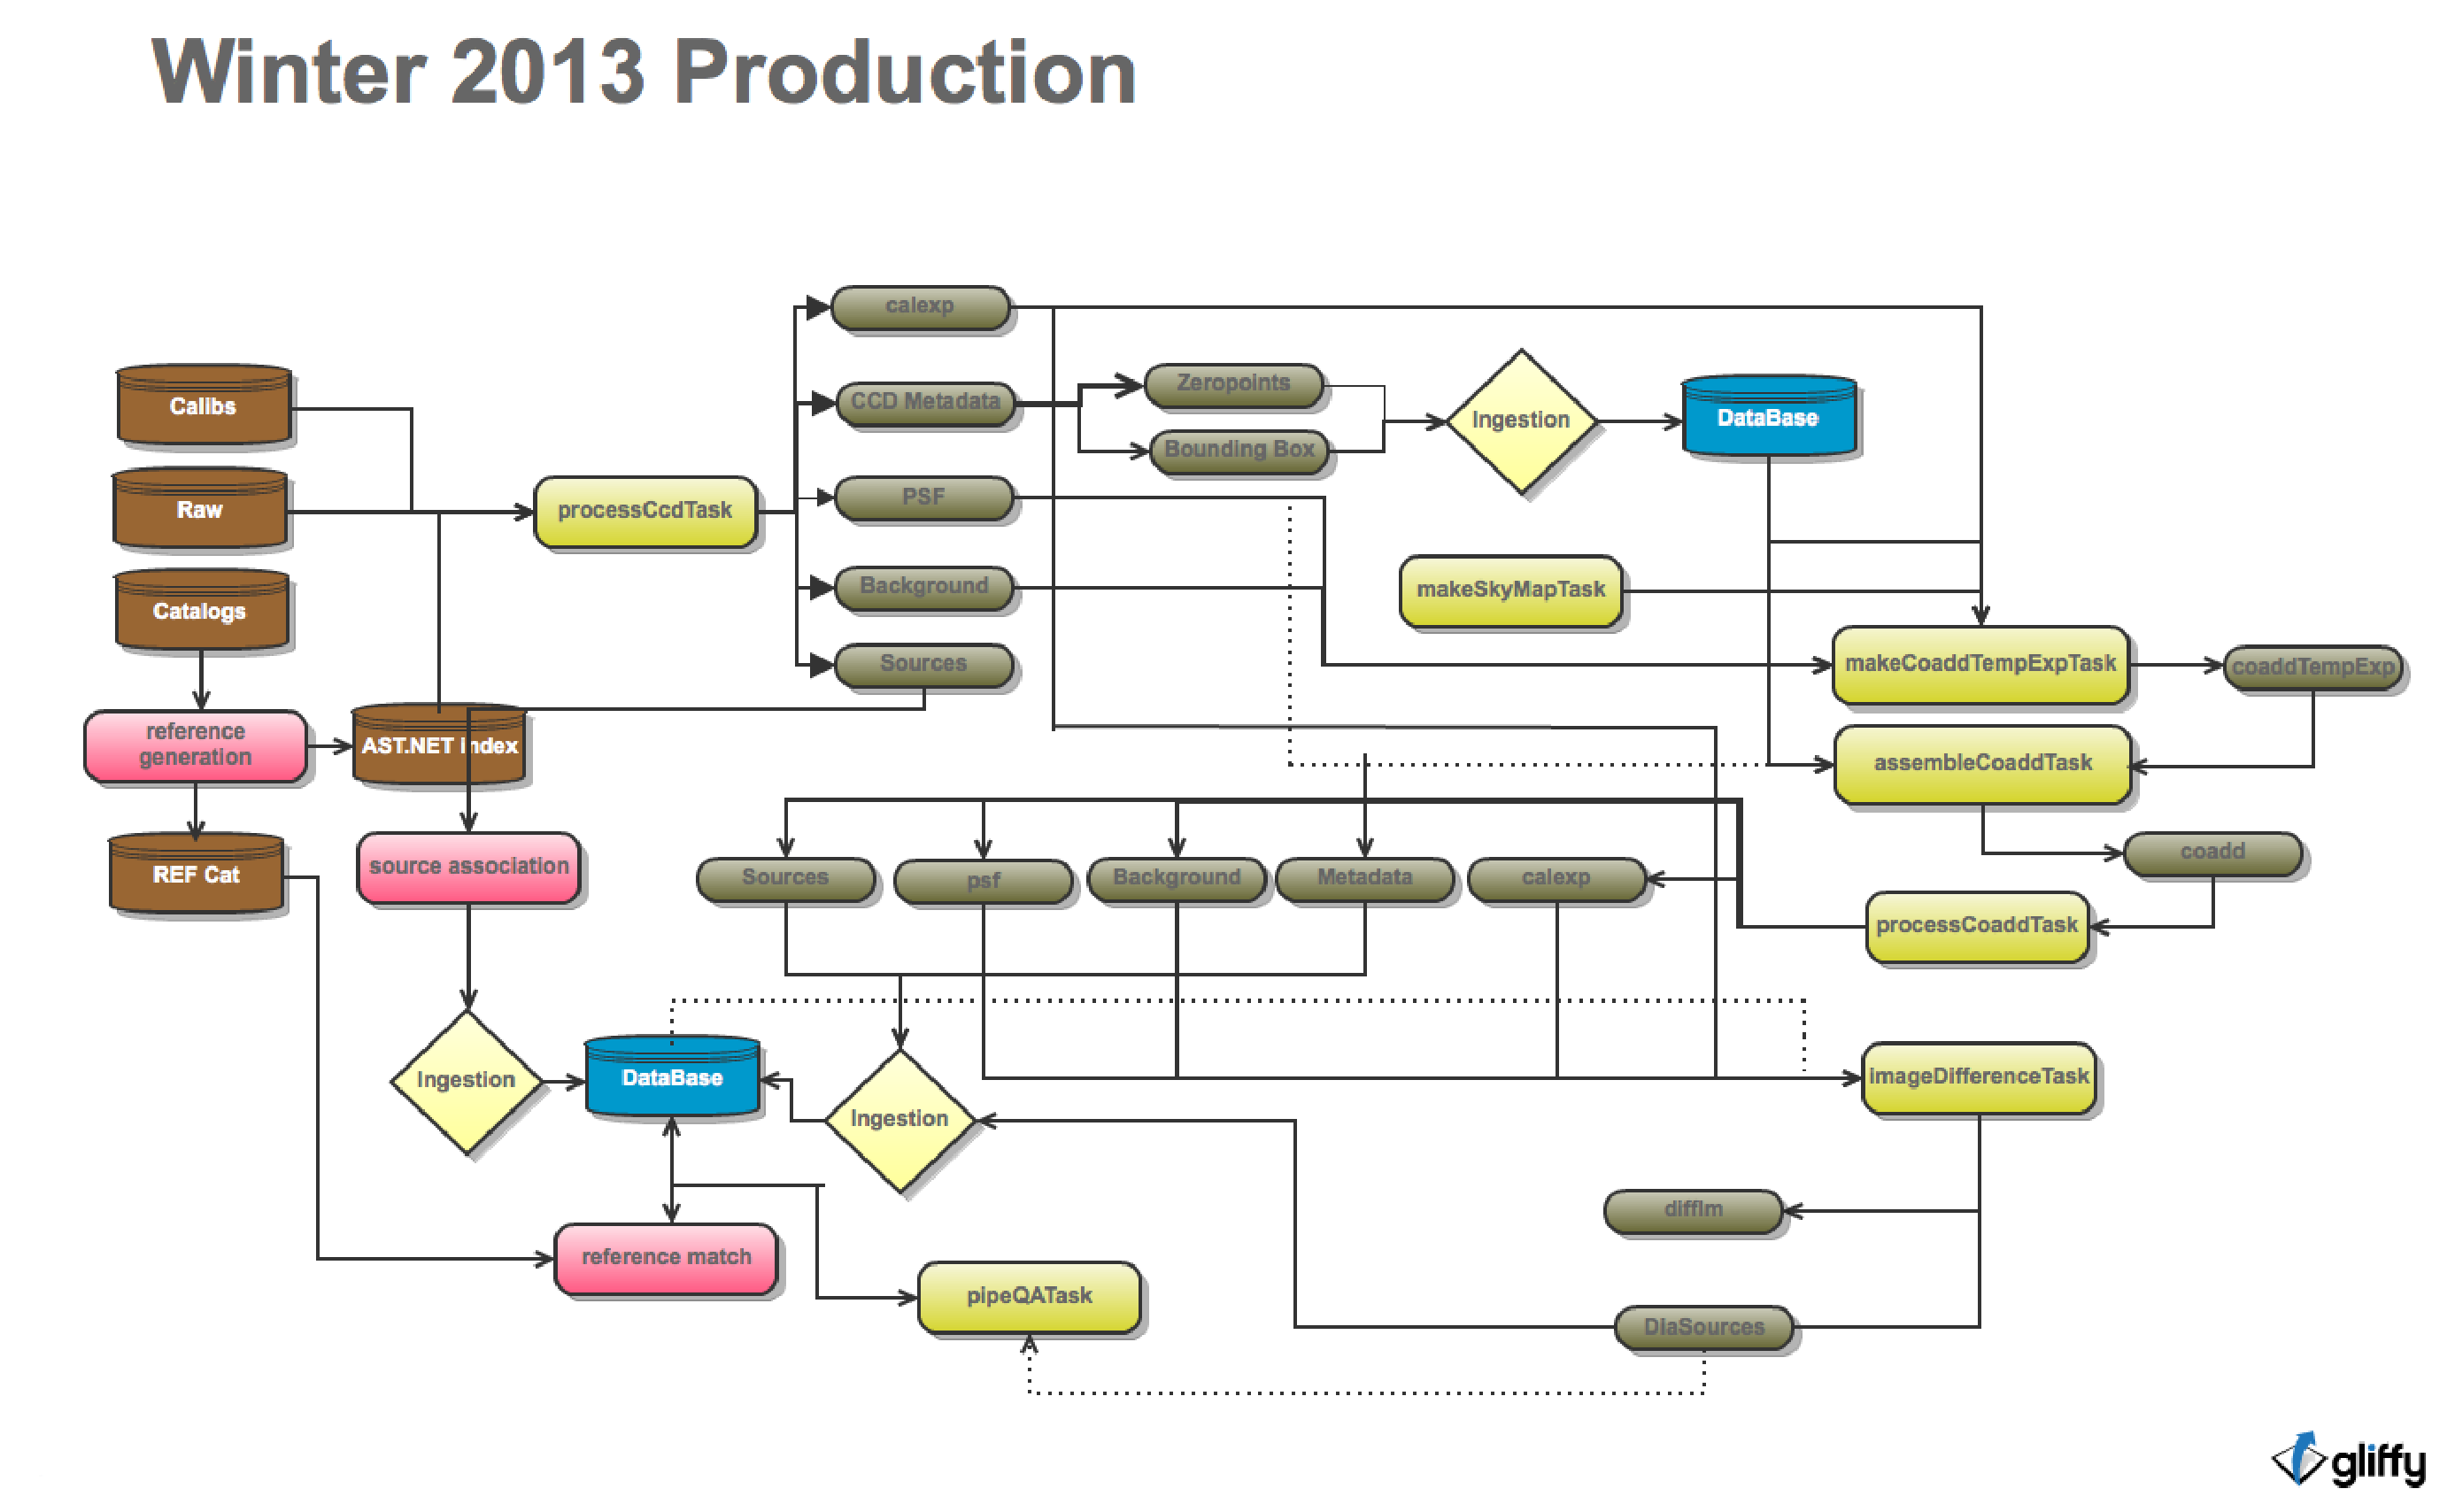
\includegraphics[height=0.7\textheight,angle=90]{flowChart.eps}

\clearpage 

\end{appendices}
%%%%%%%
%%%%%%%
%%%%%%%

\end{document}

















% Move the stuff below to above

%%%%%%%
\subsection{IsrTask (for ImSim)} \simon
Since there is no structure in the overscan, I do not believe we need
to do anything but the default for ISR.  That means overscan, bias,
flatfield, Cr interpolation, saturation and bad pixel corrections.
Right now the default for ImSim Isr is doDark=True.  This should be
fixed to reflect the fact that we no longer need dark correction with
the current model.

\subsubsection{What will be persisted}
In production we will only keep {\tt calexp}.  This means no {\tt
  postIsrCcd} will be persisted.  The Configs are automatically
persisted with the IsrTask.  Metadata to persist include: 
\begin{itemize}
\item nCR : the number of cosmic rays
\item median : the median of the calexp
\item image : 
\item gain : 
\item run time : 
\end{itemize}

\subsubsection{What is the processing time for ISR per Ccd}
The processing time is $\sim~1$ min per Ccd.

\subsubsection{What is the default Config for ISR}
\begin{python}
--config
doIsr=True
isr.doDark=False
\end{python}


\subsubsection{Which reference catalog will be used for the astrometry}

\subsubsection{Who will define it and create it from the sims}
This has been done based on the W13 surveys proposed on:
http://dev.lsstcorp.org/trac/wiki/ImSim/Summer2012Plan

\subsubsection{What depth is required for the reference catalog}
There is no reason to not go to 28$^{th}$ magnitude.  It's not that
big of an area.

\subsubsection{What format (and what processes) are required for the reference catalog}
This is very manual at the moment.  It would be nice to be able to
provide a CSV and schema to a routine that would produce both the
astrometry.net indexes and the match reach refObject.csv file.

\subsubsection{What metadata do we need to persist}
Metrics include: was the Wcs updated or did it default to the incoming
Wcs due to fitting failures; what is the RMS of the astrometric model
that was successfully fitted to the data.

\subsubsection{What is the default Config for AstrometryTask}
\begin{python}
--config
...
\end{python}




